% -----------------------------------------------
% Template for JIM
%     jim.sty -> style file
% By Eloi Batlle (eloi@iua.upf.es), changes for 
% ICMC by Bram de Jong (bdejong@iua.upf.es)
% changes for JIM 2007 by Dominique Fober (fober@grame.fr)
% changes for JIM 2009 by Olivier Tache (olivier.tache@imag.fr)
% -----------------------------------------------

\documentclass{article}
\usepackage{jim}
\usepackage[utf8]{inputenc}
\usepackage[francais]{babel}
\usepackage[T1]{fontenc}
%\usepackage{pxfonts}
\usepackage{graphicx}
\usepackage{amssymb,amsmath} 
\usepackage{balance}

\usepackage{color}
\usepackage{hyperref}
\usepackage[nocenter]{qtree}
\usepackage{tree-dvips}
\usepackage{listings}

\definecolor{lightgrey}{rgb}{0.95,0.95,0.95}
\definecolor{mycolor}{rgb}{0.0,0.0,0.8}
\hypersetup{
	colorlinks=true,
	citecolor = mycolor,
	linkcolor = mycolor,
	urlcolor  = mycolor
}

\newcommand{\IS}		{INScore}
\newcommand{\exemple}	{\vspace*{1mm}\hspace*{-4mm}\textbf{Exemple :}}

\definecolor{mygrey}{gray}{0.93}
\newcommand{\code}	[2][0.9]		{\vspace{0mm}\begin{center}\colorbox{mygrey}{
							\begin{minipage}[t]{#1\columnwidth} 
							{\small \texttt{#2}}
							\end{minipage}}\end{center}}
\newcommand{\op}	[1]		{\vspace{0mm}\begin{center}\colorbox{mygrey}{
							\begin{minipage}[t]{0.9\columnwidth} 
							{\small \texttt{#1}}
							\end{minipage}}\end{center}}
\newcommand{\nulltree}	{\ensuremath{\varnothing}}
\newcommand{\seq}		{\ensuremath{|}}
\newcommand{\paral}		{\ensuremath{\parallel}}
\newcommand{\foret}		{\ensuremath{\phi}}
\newcommand{\toforet}	{\ensuremath{\mathcal{F}}}
\newcommand{\expand}	{\ensuremath{\rightsquigarrow}}
\newcommand{\transform}	{\ensuremath{\xi}}
\newcommand{\binop}		{$op$}
\newcommand{\logop}		{$lop$}
\newcommand{\ftree}		{ftree}
\newcommand{\etc}		{…}

\newcommand{\nexpand}	{\ensuremath{\varepsilon}}
\newcommand{\ula}		{\hspace*{8mm}}
\newcommand{\ulb}		{\hspace*{4mm}}
\newcommand{\ulc}		{\hspace*{37mm}}
\newcommand{\uld}		{\hspace*{9mm}}


% Title.
% ------
\title{Un langage basé sur des arbres pour la description de partitions musicales}

% Single \textsc{address}
% To use with only one author or several with the same address
% ---------------
\oneauthor
  {D. Fober \quad Y. Orlarey \quad S. Letz \quad R. Michon} {Grame-CNCM \\
  Lyon - France \\
     {\tt {\small \{fober, orlarey, letz, michon\}@grame.fr}}}


\begin{document}
%
\maketitle
%
%-------------------------------------------------
\begin{abstract}
Le travail présenté s'inscrit dans le projet \IS, un environnement pour la conception de partition interactives augmentées, tourné vers des usages non conventionnels de la notation et de la représentation de la musique, sans exclure pour autant les approches classiques. Cet environnement est entièrement pilotable par des messages Open Sound Control [OSC]. Un langage de script, basé sur une version textuelle étendue de ces messages permet de concevoir des partitions sous forme modulaire et incrémentale. Cet article présente une révision majeure de ce langage de script, fondée sur la description et la manipulation d'arbres.
\end{abstract}

%-------------------------------------------------
\section{Introduction}\label{sec:introduction}

\IS \cite{Fober:12a} est un système de notation et de représentation de la musique initialement conçu pour être piloté par des messages OSC \cite{OSC}. Une version textuelle de ces messages a rapidement constitué le format de stockage des partitions, qui sera étendu en un langage de script \cite{Fober:13b} permettant une plus grande souplesse dans la description des partitions et des interactions avec ces partitions.

Ces extensions (introduction de variables, d'adresses étendues, section Javascript, etc.) ont néanmoins souffert d'une rigidité inhérente à une conception ad hoc et incrémentale. De ce fait, une révision majeure de ce langage nous a semblé nécessaire. Elle est basée sur la structure même du modèle d'\IS, qui est un arbre à un instant donné. 
La figure \ref{tree1} en donne un exemple, qui peut se décrire dans le langage de script actuel (soit en OSC) en énumérant toutes les branches à partir de la racine (figure~\ref{script1})
\begin{figure}[htbp]
\code{/ITL/scene/obj1 x 0;\\
/ITL/scene/obj1 y    0;\\
/ITL/scene/obj1 date 0;\\
/ITL/scene/obj2 x    0.5;\\
/ITL/scene/obj2 y    0.5;\\
/ITL/scene/obj2 date 1;
}
\caption{Script qui décrit la partition en figure \ref{tree1}.}
\label{script1}
\end{figure}


\begin{figure}[htbp]
\begin{center}
\Tree [ .ITL [ .scene 
	[ .obj1 [ .x 0 ] [ .y 0 ] [ .date 0 ] ] 
	[ .obj2 [ .x 0.5 ] [ .y 0.5 ] [ .date 1 ] ] ] 
]
\caption{Exemple d'une partition \IS\ comprenant 2 objets $obj1$ et $obj2$, qui possèdent des attributs $x$, $y$, et $date$. Les feuilles de l'arbre sont les valeurs des attributs.}
\label{tree1}
\end{center}
\end{figure}

Le langage de script d'\IS\ a donc été repensé com-me un langage de description et de manipulation d'arbres, transformable en messages OSC équivalents.

Dans la pratique, il est difficile de comparer cette approche avec les travaux existants: il existe un grand nom-bre de langage de description de partitions musicales (lilypond \cite{lilypond03}, guido \cite{hoos98}, MuseData \cite{Hewlett97}, MEI \cite{Roland_2002}, MusicXML \cite{good01}, abc \footnote{\url{http://abcnotation.com/}}, etc.) qui sont tous tournés vers la notation traditionnelle, et n'ont pas de capacité de programmation. 

L'extension de certains de ces langages a toutefois été considérée, afin de leur ajouter de la \textit{programmabilité}. Il s'agit par exemple d'opérations de composition de partitions musicale dans guido \cite{fober12b}, ou encore du langage scheme qui vient en extension de lilypond.

Il y a par ailleurs des approches résolument tournées vers la programmation avec les langages CMN \cite{Schottstaedt97} ou encore ENP 
\cite{KUUSK06} qui sont en fait des dialectes basés sur Lisp, qui adoptent principalement vers une approche classique de la notation musicale.

OSC est définit comme un protocole de communication. Des capacités de programmation ont été ajoutées \cite{429}, sous forme de \emph{fonctions} embarquables dans des messages OSC, permettant une communication structurée fonctionnelle entre applications musicales \cite{bresson:hal-01353794}. 

Aucune de ces approches ne couvre l'angle très particulier que nous avons adopté : celui d'un langage de description de partitions musicales basé sur la structure hiérachique à la fois de la partition et des messages OSC.

Après quelques définitions, nous présenterons les opérations élémentaires sur les arbres ainsi que la grammaire correspondante. Nous introduirons ensuite les opérations mathématiques sur les arbres, les concepts de \emph{variables} et de \emph{nœuds en intention} et nous présenterons enfin la transformation de ce langage en messages OSC classiques.



%-------------------------------------------------
\section{Définitions}

En théorie des graphes, un arbre enraciné ou une arborescence est un graphe acyclique orienté possédant une unique racine, et tel que tous les nœuds sauf la racine ont un unique parent. 

Un arbre sans nœuds sera appelé un \emph{arbre vide} et sera représenté par \nulltree. Un arbre non vide est constitué d'un noeud racine et potentiellement de plusieurs niveaux de nœuds supplémentaires qui forment une hiérarchie..


%---------------------------
\subsection{Terminologie}

\begin{description}
 \setlength\itemsep{0.0em}
\item[Racine]	Le nœud supérieur d'un arbre.
\item[Enfant]	Un nœud directement connecté à un autre en s'éloignant de la racine.
\item[Parent]	La notion inverse d’enfant.
\item[Feuille]	Un nœud sans enfant.
%\item[Degré]	Pour un nœud donné, son nombre d'enfants. Une feuille est nécessairement de degré zéro.
\item[Arête]	La connexion entre un nœud parent et un nœud enfant.
\item[Chemin]	La séquence de nœuds et d’arêtes reliant un nœud à un descendant.
\item[Forêt]	Un ensemble de $n >= 0$ arbres disjoints.
\end{description}

%---------------------------
\subsection{Arbres}
Un arbre est définit par une valeur et l’ensemble de ses sous-arbres (i.e. une forêt):
\code{f := [ t[1],..., t[k] ] \\
t :=  v f
}



%-------------------------------------------------
\section{Operations sur les arbres}

%-----------------------------
\subsection{Mise en séquence}
Nous noterons \seq\ l'opération de mise en séquence de 2 arbres. \\
Soit 2 arbres \texttt{t} et \texttt{t'} définis comme suit :
\op{f := [ t[1],\etc, t[k] ] \\
t :=  v f \\
\\
f' := [ t'[1],\etc, t'[k] ] \\
t' :=  v' f'
}
alors
\op{t \seq\ t'  $\Rightarrow$  t" := v f" \\
f" := [ t[1] \seq\ t',\etc, t[k] \seq\ t']
}
avec : 
\op{t :=  v [ \nulltree\ ]\\
t \seq\ t'  $\Rightarrow$  t" := v [ t' ]
}


%-----------------------------
\subsection{Mise en parallèle}
Nous noterons \paral\ l'opération de mise en parallèle. 
Soit 2 arbres $t$ et $t'$ :
\op{t \paral\ t'  $\Rightarrow$  t": \foret\ [ t, t' ]
}
\texttt{t"} est un arbre dont la valeur \foret\ symbolise une forêt. 

Nous nommerons \emph{\ftree} le type d'arbre dont la valeur est \foret\ et nous étendons l'opération de mise en séquence aux \emph{\ftree}\ de la manière suivante. Soit un \emph{\ftree} $t'$~ :
\op{t' :=  \foret\ f\\
t \ :=  v [ \nulltree\ ]\\
\\
t \seq\ t'  $\Rightarrow$  t" := v f
}

L'opération de mise en parallèle appliquée à un \emph{\ftree} est distribuée aux enfants : 
\op{t :=  \foret\ [ t[1],\etc, t[k] ]\\
t' :=  v f\\
\\
t \paral\ t'  $\Rightarrow$  t" := \foret\ [t[1],\etc,t[k], t']\\
t' \paral\ t  $\Rightarrow$  t" := \foret\ [t', t[1],\etc,t[k]]
}



%-------------------------------------------------
\section{Grammaire}\label{agram}

Un arbre est syntactiquement définit comme suit :
\code{tree := value      \hspace*{8mm} $\to$ t := value [ \nulltree ] \\
\ula | tree tree         \hspace*{4mm} $\to$ t := tree \seq\ tree \\
\ula | / tree            \hspace*{9.7mm} $\to$ t := '/' \seq\ tree\\
\ula | tree , tree       \hspace*{0mm}  $\to$ t := tree \paral\ tree \\
\ula | ( tree )          \hspace*{6mm} $\to$ t := tree \\
\ula ;\\
}

\exemple

La figure~\ref{parsesample1} donne un exemple de cette grammaire et de l'arbre construit par ce script. La figure~\ref{treesample1} présente ce même arbre après évaluation des opérations de mise en séquence ($seq$) et en parallèle ($par$).

\begin{figure}[htbp]
\code{/a/b (c, (d e), f) (x 0), (y 1)}
\begin{center}
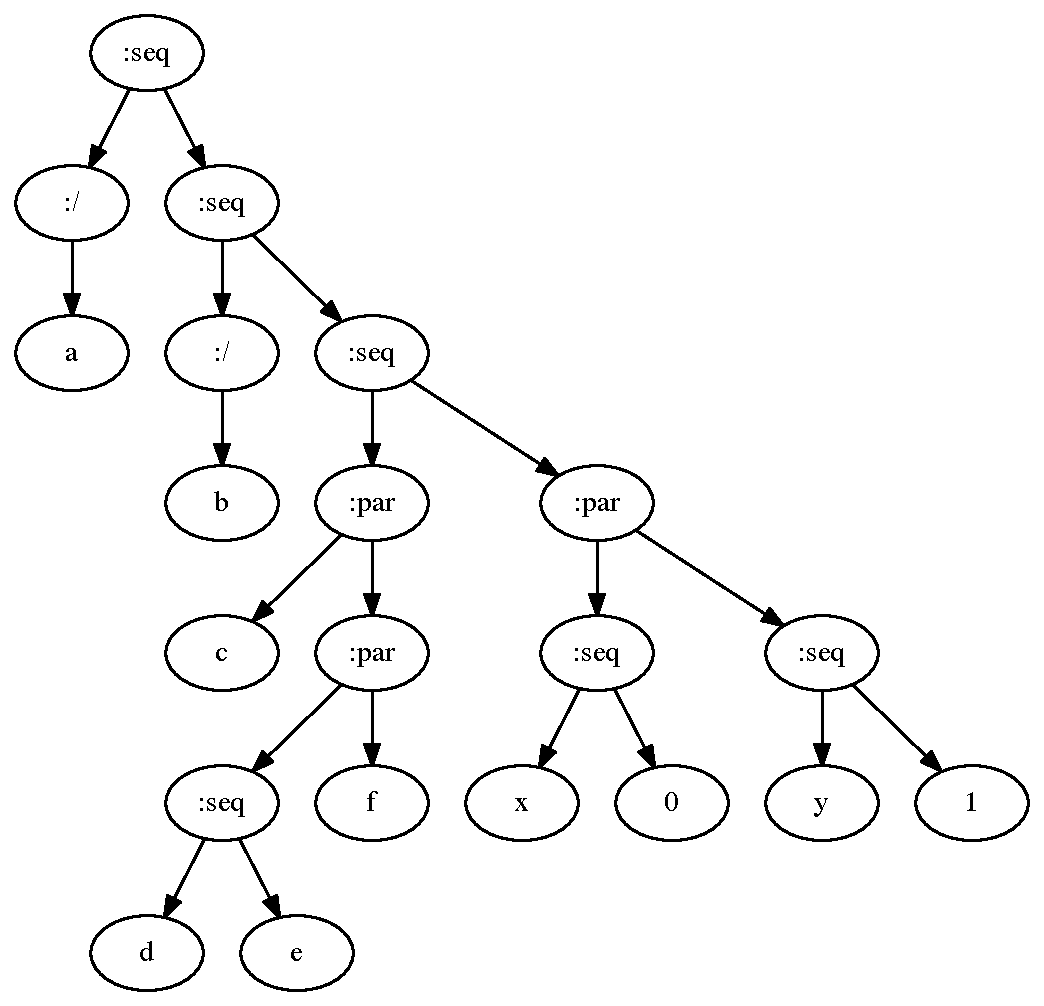
\includegraphics[width=0.9\columnwidth]{parse/sample1}
\caption{Arbre construit par le script en ci-dessus.}
\label{parsesample1}
\end{center}
\end{figure}

\begin{figure}[htbp]
\begin{center}
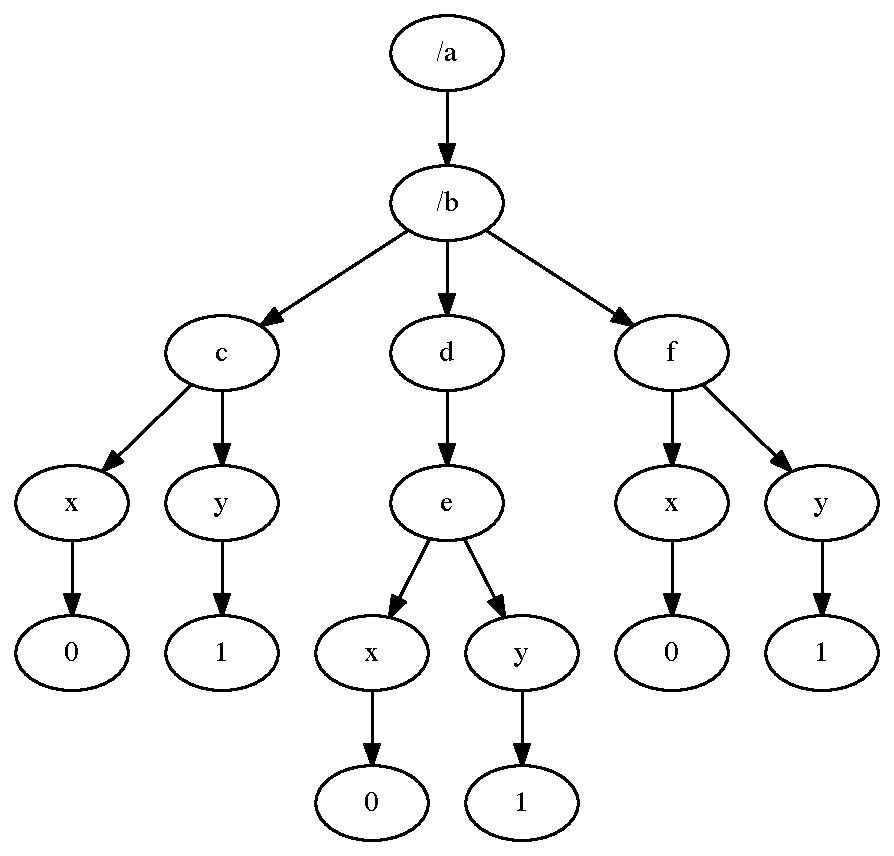
\includegraphics[width=0.8\columnwidth]{eval/sample1}
\caption{Arbre généré après évaluation des opérations de mise en séquence ($seq$) et en parallèle ($par$) de l'arbre en figure \ref{parsesample1}.}
\label{treesample1}
\end{center}
\end{figure}

Les nœuds dont la valeur est \emph{slash} (/) jouent un rôle particulier dans la transformation de arbre en messages OSC. Ce rôle est décrit en section \ref{ssec:slash}.


%-------------------------------------------------
\section{Valeurs et évaluation}\label{sec:valeurs}

Les noeuds d'un arbre peuvent contenir des valeurs littérales (texte, nombre) ou des valeurs spéciales qui sont parmi les types suivants:
\begin{itemize}
\item opérateurs mathématiques
\item variables
\item nœuds en intention
\item slash (/)
\end{itemize}


%---------------------------
\subsection{Opérateurs mathématiques}

Les opérations mathématiques sur des arbres sont vues comme des opérations qui portent sur leurs valeurs tout en conservant les sous-arbres. Ces opérations sont parmi :
\begin{itemize}
\item opérations arithmétiques (+ - * / \%)
\item opérations logiques ($==$ $<$ $\leq$ $>$ $\geq$)
\item fonction trigonométriques (sin, cos, tan, asin, acos, atan)
\item fonction hyperboliques (sinh, cosh, tanh, asinh, acosh, atanh)
\item fonctions exponentielles et logarithmiques (exp, log, log10, log2)
\item puissances (pow, sqrt, cbrt)
\item fonctions diverses (min, max, rand)
\end{itemize}

Nous désignerons ces opérations par \binop. Soit alors :
\op{t :=  v f\\
t' := v' f'\\
\binop\ t t'  $\Rightarrow$  t":  (\binop\ v v') [ f $\cup$ f' ]  
}

\exemple

Le script en figure~\ref{parsesample2} genère l'arbre illustré en figure \ref{treesample2} après évaluation des opérations mathématiques.

\begin{figure}[htbp]
\code{/a/b 	(c ((* (math.sin 1), 2)) 1) ,\\
\ulb		(d (math.pow 2.2, 0.4)),\\
\ulb		(e (>= 1, 1) (math.max 1, 2, 3, 4));}
\begin{center}
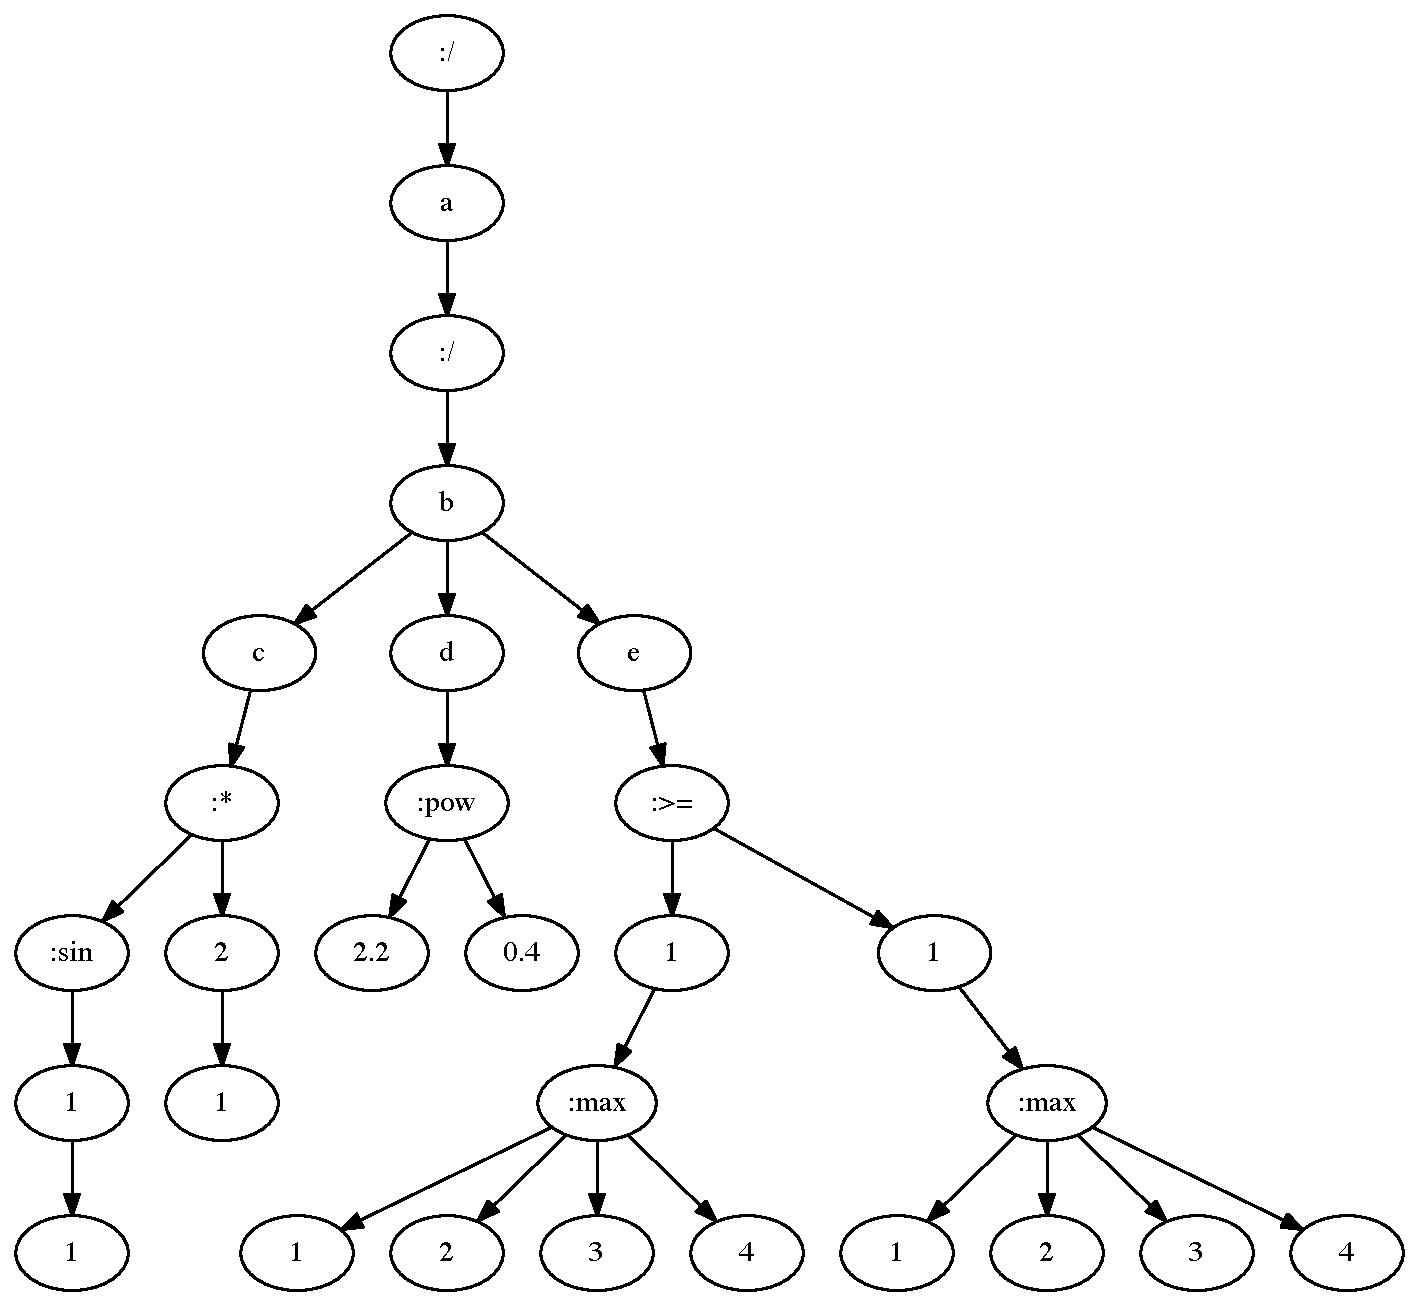
\includegraphics[width=1\columnwidth]{tree/sample3}
\caption{Arbre construit par le script ci-dessus.}
\label{parsesample2}
\end{center}
\end{figure}

\begin{figure}[htbp]
\begin{center}
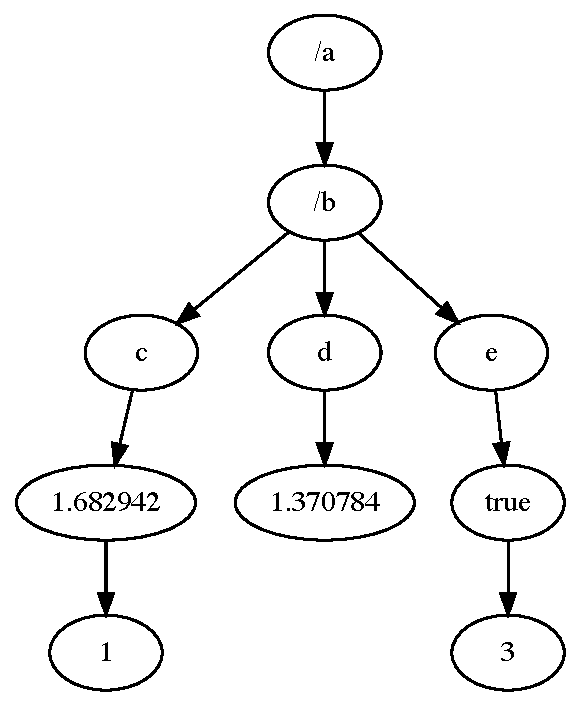
\includegraphics[width=0.5\columnwidth]{eval/sample3}
\caption{Arbre généré après évaluation des opérations mathématiques de l'arbre en figure \ref{parsesample2}.}
\label{treesample2}
\end{center}
\end{figure}


%---------------------------
\subsubsection{Sélecteurs}

Un sélecteur est un arbre qui prend la forme suivante :
\code{? condition, if\_true, if\_false}
Il sélectionne une des deux branches en fonction de la valeur booléenne de la \emph{condition}.

\pagebreak
\exemple

Une fois évalué, le script illustré en figure~\ref{dotselect} sera réduit à l'arbre $t := 1\ [\nulltree]$.

\begin{figure}[htbp]
\code{? true, 1, 0;}
\begin{center}
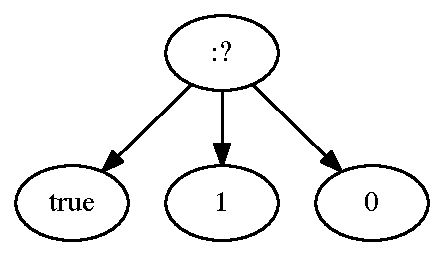
\includegraphics[width=0.4\columnwidth]{tree/select}
\caption{Arbre construit par le sélecteur ci-dessus. En regard de la valeur du premier enfant, son évaluation va sélectionner la branche 1.}
\label{dotselect}
\end{center}
\end{figure}



%---------------------------
\subsection{Variables}

Une variable est l’association d'un identifiant et d’un arbre. Sa forme générale est 
$varname = t$

\exemple
\code{foo = /A/B (x 0), (y 1); }

%---------------------------
\subsubsection{Evaluation}

L'évaluation d'une variable consiste à expanser l'arbre représenté par cette variable à sa position courante.
Soit un arbre $t$ et une variable $var$ définis comme suit :
\op{t :=  v f\\
var = t
}
L'évaluation de $var$ dans le contexte d'un arbre $t'$ est définie comme suit :
\op{t'$_{\{var\}}$ :=  \$var f' $\Rightarrow$ t" := t \seq\ \toforet(t') \\
où \\
\toforet(t := v f) $\Rightarrow$ t' := \foret\ f
}
t'$_{\{var\}}$ désigne un arbre dont l'environnement contient la variable $var$.


\exemple
\code{x = x 0;\\
y = y 0;\\
/A/B \$x, \$y; \ \ $\Rightarrow$  /A/B (x 0), (y 1);}


%---------------------------
\subsubsection{Environnement local à une variable}

Chaque arbre est évalué dans un environnement constitué de la liste de toutes les variables de son parent. Une variable peut-être évaluée dans un environnement qui lui est local :
\code{var = t;\\
\\
\$var\{a=t1, b=t2,\etc\} \ \ $\Rightarrow$  t' := t$_{\{a, b,\etc\}}$}


%---------------------------
\subsection{Nœuds en intention}

Les nœuds en intention sont une forme compacte de description d'une forêt. On peut les voir également comme une manière de décrire des boucles. Leur forme générale est la suivante :
\begin{description}
\item $id[n…m]$ 	où $n$ et $m$ sont des entiers
\item $id[ab…xy]$ où $a,b,x,y$ sont des lettres.
\end{description}

L'expansion d'un nœud en intention consiste à transformer ce nœud en une forêt. Nous noterons \nexpand\ l'opération d'expansion :
\code{\nexpand(id[n…m]) \ $\Rightarrow$ \foret [id$n$,id$n+1$,…,id$m$]\\
\\
\nexpand(id[ab…xy]) $\Rightarrow$ \foret [id$ab$,id$ac$,…,id$ay$,\\
\ulc id$bb$,id$bc$,…,id$by$,\\
\ulc …,\\
\ulc id$xb$,id$xc$,…,id$xy$]
}

%---------------------------
\subsubsection{Formes particulières}

Les nœuds en intention peuvent prendre les formes particulières suivantes : 
\begin{description}
\item $id[i:n…m]$ 	où $i$ est un identificateur
\item $id[i:j:ab…xy]$ où $i,j$ sont des identificateurs.
\end{description}
Ces identificateurs désignent des variables qui sont instanciées dans l'environnement par l'opération d'expansion, avec la valeur d'indice courante :
\code{\nexpand(id[i:n…m]) \\
\ $\Rightarrow$ \foret [id$n_{\{i=0\}}$,id$n+1_{\{i=1\}}$,…,id$m_{\{i=m-n\}}$]\\
\\
\nexpand(id[i:j:ab…xy]) \\
\ $\Rightarrow$ \foret [id$ab_{\{i=0,j=0\}}$,…,id$ay_{\{i=y-b,j=0\}}$,\\
\uld id$bb_{\{i=0,j=1\}}$,…,id$by_{\{i=y-b,j=1\}}$,\\
\uld …,\\
\uld id$xb_{\{i=0,j=x-a\}}$…,id$xy_{\{i=y-b,j=x-a\}}$]
}

\exemple

Le script illustré en figure~\ref{parsesample3} genère l'arbre illustré en figure \ref{treesample3} après expansion et évaluation des variables et des opérations mahématiques :

\begin{figure}[htbp]
\code{/a/b[i:1...3] x (- (* \$i, 0.5), 0.5);}
\begin{center}
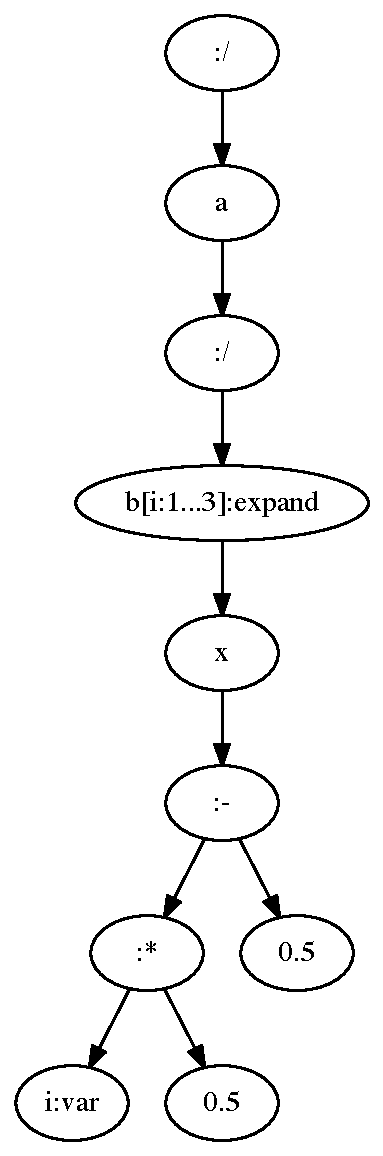
\includegraphics[width=0.35\columnwidth]{tree/sample2}
\caption{Arbre construit par le script ci-dessus}
\label{parsesample3}
\end{center}
\end{figure}

\begin{figure}[htbp]
\begin{center}
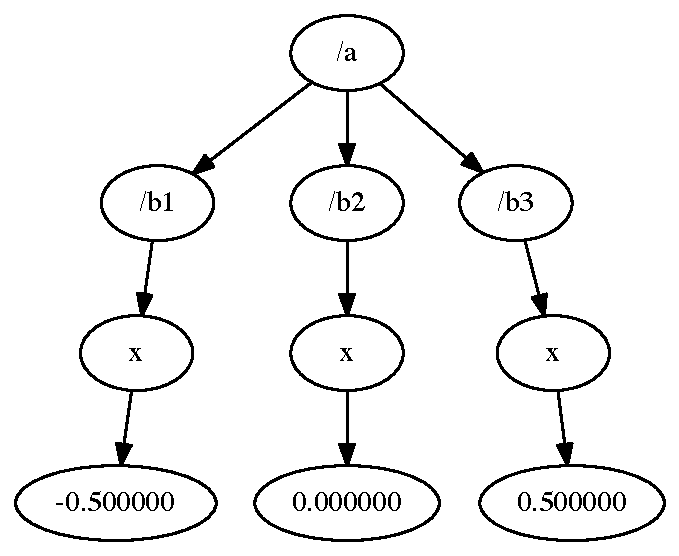
\includegraphics[width=0.6\columnwidth]{eval/sample2}
\caption{Arbre généré par l'expansion et évaluation des variables et des opérations mathématiques de l'arbre en figure \ref{parsesample3}.}
\label{treesample3}
\end{center}
\end{figure}


%---------------------------
\subsection{Slash (/)}\label{ssec:slash}

Les nœuds \emph{slash} sont utilisés pour la transformation d'un arbre en messages OSC et notamment pour discriminer l'adresse OSC des paramètres du message. La transformation d'un arbre en messages OSC consiste à énumérer tous les chemins à partir de la racine jusqu'au premier paramètre. Le premier paramètre est le premier nœud qui n'est pas précédé d'un \emph{slash}.

\exemple

Le script suivant construit l'arbre illustré en figure~\ref{evalsample4}. Sa transformation au format OSC est illustrée en figure~\ref{pathssample4}.
\begin{figure}[htbp]
\code{/a/b (set txt "Hello"),\\
\uld	 (color 1, 2, 3);
}
\begin{center}
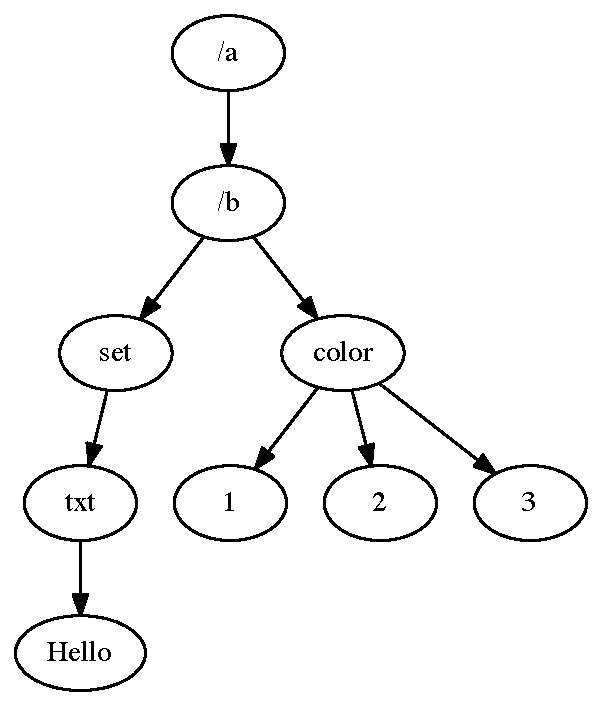
\includegraphics[width=0.6\columnwidth]{eval/sample4}
\caption{Arbre construit par le script ci-dessus.}
\label{evalsample4}
\end{center}
\end{figure}

\begin{figure}[htbp]
\begin{center}
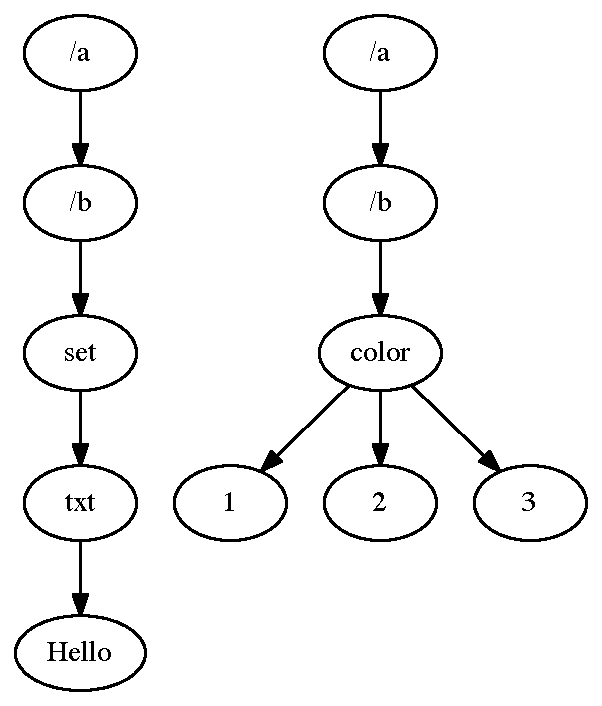
\includegraphics[width=0.6\columnwidth]{paths/sample4}
\caption{Transformation de l'arbre de la figure \ref{evalsample4} en chemins OSC.}
\label{pathssample4}
\end{center}
\end{figure}


%-------------------------------------------------
\section{Exemple de script}

Le script ci-dessous présente un exemple de cette nouvelle version du langage \IS . Les variables sont indiquées en bleu, les variables locales sont déclarées en rouge.


\lstdefinelanguage{inscore} 
{
classoffset=0,
morekeywords={}, keywordstyle=\color{blue},
classoffset=1,
morekeywords={addr, count, radius, size, pos, color }, keywordstyle=\color{red},
classoffset=2,
keywordsprefix=$,
sensitive=true,
morecomment=[l]{\#},
morestring=[b]", 
}

\lstset{backgroundcolor=\color{lightgrey}, extendedchars=true, inputencoding=utf8}

\begin{lstlisting}[language=inscore, extendedchars=true, basicstyle=\small\ttfamily]
# variables declaration 
pi    = 3.141592653589793;

# the next variables make use of 'count'
# a variable that is instanciated locally
step  = / ( * 2, $pi), $count;
hstep = / 0.3, $count;

x = math.sin ( * $step, (+ $i, $pos));
y = math.cos ( * $step, (+ $i, $pos));

hue    = (+ $color, (* $hstep, $i));
bstart = 0.4;
bstep  = / (- 1, $bstart), $count;
brigthness= + $bstart, (* $bstep, $i);

# this is a classical OSC message
# that simply clears the scene
/ITL/scene/* del;

# this is the main variable. It will be
# expanded to create a series of objects.
# Most of the variables are locally defined.  
circle = (/ITL/scene/$addr  
          (set ellipse $size $size),
          (x * $x, $radius),
          (y * $y, $radius),
          (hsb $hue, $brigthness,1.));

# finally the 'circle' variable is used
# with different parameters. 
$circle{addr=c1_[i:1...30],count=30, 
   radius=0.7,size=0.1,pos=0,color=0.};
$circle{addr=c2_[i:1...24],count=24,
   radius=0.5,size=0.08,pos=6,color=0.1};
$circle{addr=c3_[i:1...20],count=20,
   radius=0.3,size=0.06,pos=10,color=0.2};
$circle{addr=c4_[i:1...12],count=12,
   radius=0.15,size=0.045,pos=9,color=0.35};

\end{lstlisting}



L'évaluation de ce script produit des messages OSC pleinement compatibles avec la version précédente du langage et qui sont schématiquement présentés ci-dessous. 
\code[1]{/ITL/scene/c1\_1 set ellipse 0.1 0.1;\\
/ITL/scene/c1\_1 x 0.0;\\
/ITL/scene/c1\_1 y 0.7;\\
/ITL/scene/c1\_1 hsb 0.0 0.4 1.;\\
/ITL/scene/c1\_2 set ellipse 0.1 0.1;\\
/ITL/scene/c1\_2 x 0.145538;\\
/ITL/scene/c1\_2 y 0.684704;\\
/ITL/scene/c1\_2 hsb 0.01 0.42 1.;\\
...\\
...\\
/ITL/scene/c4\_12 set ellipse 0.045 0.045;\\
/ITL/scene/c4\_12 x -0.129904;\\
/ITL/scene/c4\_12 y -0.074999;\\
/ITL/scene/c4\_12 hsb 0.625 0.95 1.;
}


Dans la pratique, cet exemple (illustré par la figure \ref{samplescene}) exprime en 20 lignes, les 345 lignes équivalentes et nécessaires dans la version précédente du langage.

\begin{figure}[htbp]
\begin{center}
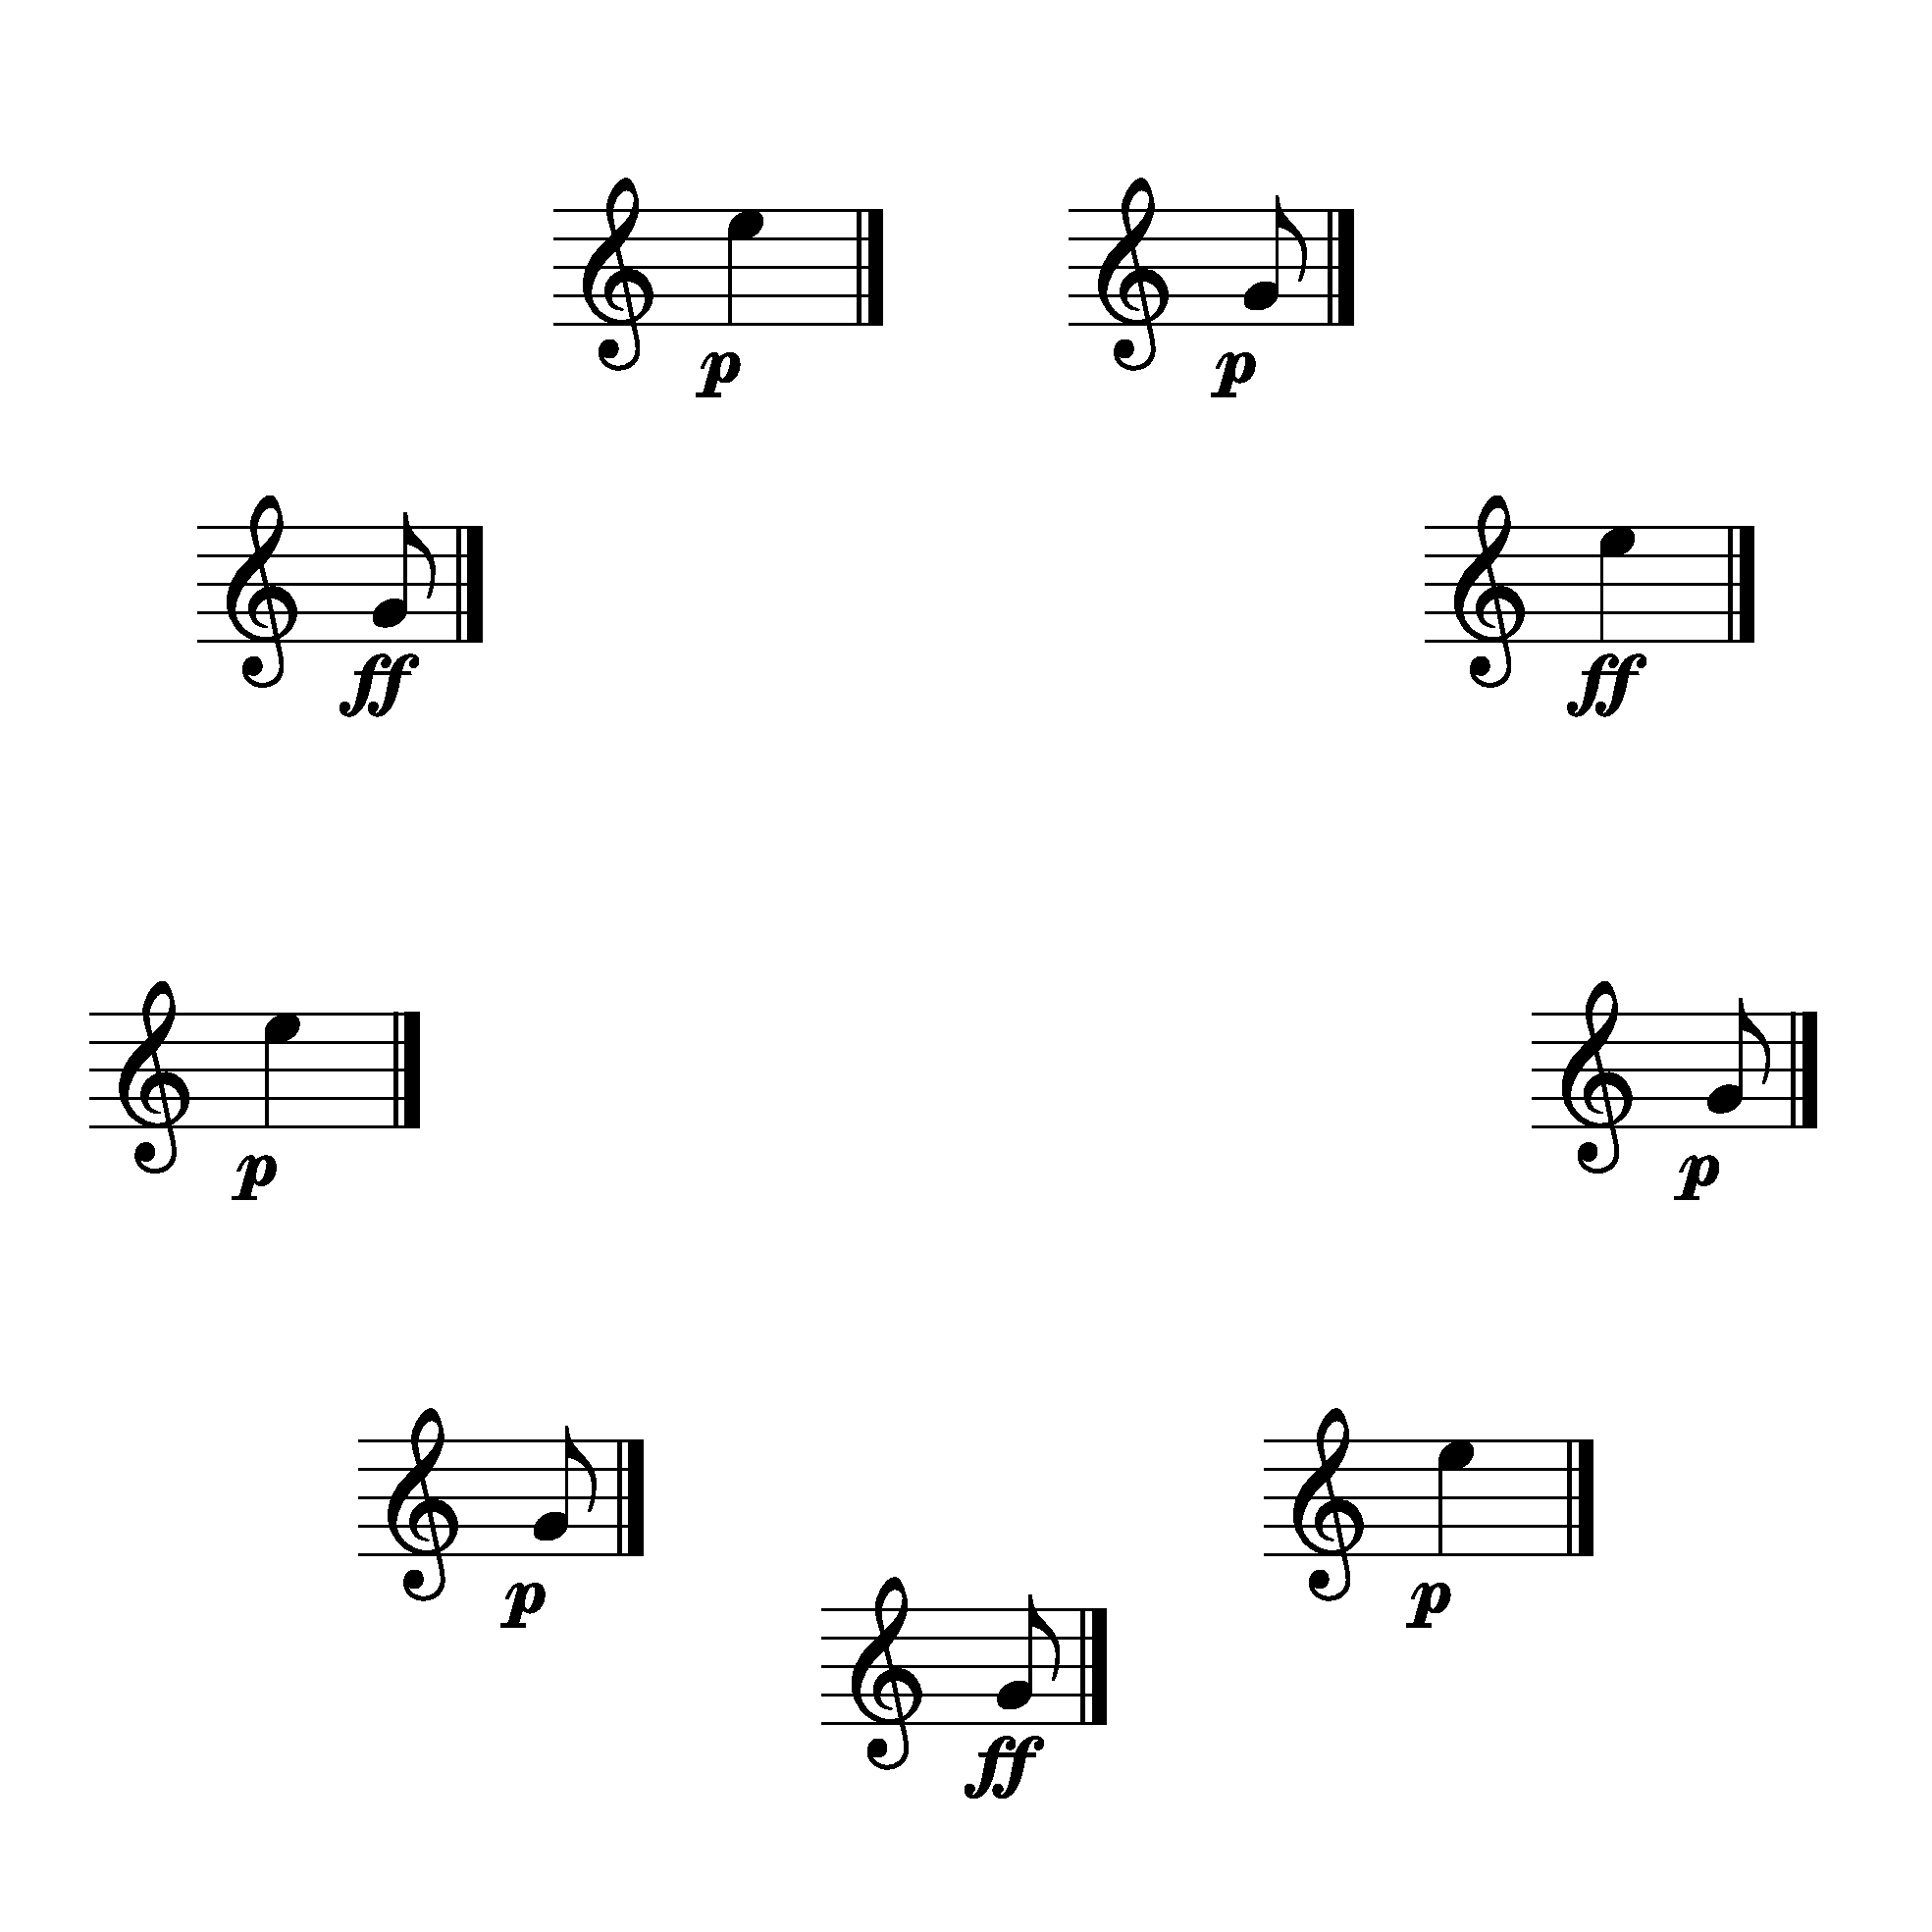
\includegraphics[width=0.9\columnwidth]{scene}
\caption{Partition \IS\ correspondant au script ci-dessus.}
\label{samplescene}
\end{center}
\end{figure}


%==============================================================
\section{Conclusion}

A partir de deux opérations élémentaires sur des arbres - la mise en séquence et en parallèle -, nous avons pu introduire de manière homogène, les notions de variables et d'opérations mathématiques et logiques portant sur des arbres. Le langage résultant est d'une  expressivité sans commune mesure avec la version précédente du langage de script d'\IS . Il permet notamment la mise en parallèle des arguments d'un message, d'utiliser des variables pour décrire des adresses, d'exprimer des séries d'adresses de manière concise, et d'utiliser des variables locales permettant la réutilisation de scripts ou de parties de scripts dans des contextes différents.

\balance
\bibliographystyle{plain}
\bibliography{../interlude}


\end{document}
